\documentclass{article}
% translate with >> pdflatex -shell-escape <file>

\usepackage{pgfplots}
\pgfplotsset{compat=newest}

\pagestyle{empty}

\begin{document}
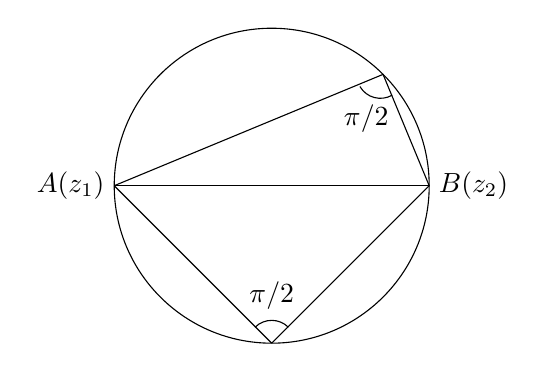
\begin{tikzpicture}%
            \draw (0, 0) circle(2);
            \draw (-2, 0) -- (2, 0);
            \draw (-2, 0) -- (1.414, 1.414) (2, 0) -- (1.414, 1.414) (-2, 0) --
            (0, -2) (2, 0) -- (0, -2);
            \draw (-2, 0) node[anchor=east] {$A(z_1)$} (2,
            0) node[anchor=west] {$B(z_2)$};
            \draw (1.53, 1.15) arc(300:210:.3);
            \draw(.2121, -1.7979) arc(45:135:.3);
            \draw (1.2, 1.15) node[anchor=north] {$\pi/2$} (0, -1.7)
            node[anchor=south] {$\pi/2$};
\end{tikzpicture}%
\end{document}

